\chapter{Objektverfolgung}

Dieses Kapitel beschreibt, wie die zuvor extrahierten Detektionen über die Zeit hinweg zu konsistenten Objektspuren zusammengeführt werden. Der Fokus liegt auf dem zweidimensionalen Kalman-Filter mit passendem Bewegungsmodell, der Mess- und Zuordnungslogik mittels Ungarischem Algorithmus sowie dem Track-Management. Abschließend werden die Testschritte und die beobachtete Stabilität der Track-IDs zusammengefasst.

\section{Prinzip}

Kern des Trackers ist ein zweidimensionaler Kalman-Filter, der Positions- und Geschwindigkeitsanteile in der Straßenebene fortschreibt und bei neuen Messungen aktualisiert. Jeder Tracking-Zyklus durchläuft denselben Ablauf: (1) \textbf{Prädiktion} aller bestehenden Tracks anhand des Bewegungsmodells, (2) \textbf{Gating} der eingehenden Detektionen über Mahalanobis-Distanzen, (3) \textbf{globale Zuordnung} der verbleibenden Paare per Ungarischem Algorithmus sowie (4) \textbf{Track-Management}. Dieses verwaltet Neuinitialisierungen aus nicht zugeordneten Detektionen, lässt bestehende Tracks für eine begrenzte \textit{Time-to-Live} ohne Messung weiterlaufen und entfernt überalterte Spuren. Die Beschränkung auf die 2D-Ebene reduziert den Rechenaufwand, da Höhenvariationen bereits in der Clustering-Stufe bewertet werden. Die folgenden Abschnitte erläutern Kalman-Filter und Zuordnungslogik im Detail.

\subsection{2D-Kalman-Filter}
Der Kalman-Filter schätzt den Zustandsvektor eines Objekts und aktualisiert ihn bei jeder neuen Messung (\cite{kalman1960}). Im hier verwendeten 2D-Modell lautet der Zustandsvektor
\[
\mathbf{x} =
\begin{bmatrix}
x \\ y \\ v_x \\ v_y
\end{bmatrix},
\]
wobei $(x,y)$ die Position und $(v_x, v_y)$ die Geschwindigkeit in der Ebene beschreiben. Als Bewegungsmodell wird konstante Geschwindigkeit angenommen, d.\,h. die Position entwickelt sich proportional zur Geschwindigkeit, während die Geschwindigkeit unverändert bleibt. Dieses lineare Modell ist für Tracking-Aufgaben im Verkehrsumfeld weit verbreitet \parencite{bar2004estimation}.

Die Zustandsvorhersage erfolgt mittels Übergangsmatrix
\[
\mathbf{F} =
\begin{bmatrix}
1 & 0 & \Delta t & 0\\
0 & 1 & 0 & \Delta t\\
0 & 0 & 1 & 0\\
0 & 0 & 0 & 1
\end{bmatrix},
\]
wobei $\Delta t$ die Zeitdifferenz zwischen zwei Messungen darstellt. Die Kovarianzmatrix wird entsprechend
\[
\mathbf{P}_{k|k-1} = \mathbf{F}\,\mathbf{P}_{k-1|k-1}\,\mathbf{F}^T + \mathbf{Q}
\]
fortgeschrieben, wobei $\mathbf{Q}$ das Prozessrauschen modelliert und Beschleunigungen oder Modellabweichungen abdeckt. In der Implementierung wird $\mathbf{Q}$ auf Basis der empirisch beobachteten Geschwindigkeitsänderungen gewählt (typisch $\sigma_a \approx 1\,\mathrm{m/s^2}$), um kurzfristige Manöver abzufangen, ohne dass der Filter instabil wird.

Liegt eine neue Detektion vor, wird der Filter aktualisiert. Die erwartete Messung wird über
\[
\mathbf{z}_{k|k-1} = \mathbf{H}\,\mathbf{x}_{k|k-1}, \quad
\mathbf{H} =
\begin{bmatrix}
1 & 0 & 0 & 0\\
0 & 1 & 0 & 0
\end{bmatrix}
\]
berechnet. Der Innovationsvektor lautet
\[
\mathbf{y}_k = \mathbf{z}_k - \mathbf{H}\,\mathbf{x}_{k|k-1},
\]
und mit der Innovationskovarianz
\[
\mathbf{S}_k = \mathbf{H}\,\mathbf{P}_{k|k-1}\,\mathbf{H}^T + \mathbf{R}
\]
ergibt sich der Kalman-Gewinn:
\[
\mathbf{K}_k = \mathbf{P}_{k|k-1}\,\mathbf{H}^T\,\mathbf{S}_k^{-1}.
\]

Damit wird der Zustand korrigiert zu
\[
\mathbf{x}_{k|k} = \mathbf{x}_{k|k-1} + \mathbf{K}_k\,\mathbf{y}_k,
\]
und die Unsicherheit reduziert sich entsprechend
\[
\mathbf{P}_{k|k} = (\mathbf{I} - \mathbf{K}_k\mathbf{H})\,\mathbf{P}_{k|k-1}.
\]

Die normierte Innovationsgröße
\[
d^2 = \mathbf{y}_k^T\,\mathbf{S}_k^{-1}\,\mathbf{y}_k
\]
entspricht dem Mahalanobis-Abstand und dient als statistisches Maß, ob eine Messung konsistent zu einem Track passt. Große Abweichungen führen zur Ablehnung der Zuordnung (\textit{Gating}) (\cite{bar2004estimation}). Als Gate wird ein $\chi^2$-Schwellwert (typisch $d^2 \leq 9$ für 95~\% Konfidenz in 2D) genutzt. Nicht geupdatete Tracks behalten ihre Prädiktion, ihre Kovarianz wächst jedoch, wodurch der Gate-Radius über die Zeit zunimmt und späte Wiedererkennungen erleichtert.

\subsection{Datenassoziation mit dem Ungarischen Algorithmus}

Um in jedem Zeitschritt neue Detektionen den bestehenden Objekt-Spuren (Tracks) korrekt zuzuordnen, wird ein Zuordnungsproblem gelöst. Hierfür wird zunächst eine Kostenmatrix
\[
\mathbf{C} \in \mathbb{R}^{N_\text{Track} \times N_\text{Detektion}}
\]
aufgebaut, deren Eintrag $c_{ij}$ die Kosten einer möglichen Zuordnung zwischen Track $i$ und Detektion $j$ beschreibt. In dieser Arbeit wird als Kostenmaß der quadratische Mahalanobis-Abstand verwendet,
\[
c_{ij} = (\mathbf{z}_j - \hat{\mathbf{z}}_i)^\mathrm{T}\, \mathbf{S}_i^{-1}\, (\mathbf{z}_j - \hat{\mathbf{z}}_i),
\]
wobei $\hat{\mathbf{z}}_i$ die vom Kalman-Filter vorhergesagte Position des Tracks und $\mathbf{S}_i$ die Innovationskovarianz ist \parencite{bar2004estimation}. Kleine Werte stehen für hohe Übereinstimmung. 

Um unrealistische Paarungen auszuschließen, wird ein \textit{Gating} durchgeführt: liegt $c_{ij}$ oberhalb eines Schwellenwerts $\tau$, wird diese Zuordnung verworfen. Praktisch wird dies durch Setzen des Matrixeintrags auf einen sehr großen Wert erreicht:
\[
c_{ij} =
\begin{cases}
(\mathbf{z}_j - \hat{\mathbf{z}}_i)^\mathrm{T}\, \mathbf{S}_i^{-1}\, (\mathbf{z}_j - \hat{\mathbf{z}}_i), & \text{falls } c_{ij} \le \tau,\\
\infty, & \text{sonst}.
\end{cases}
\]
Dadurch werden nur Messungen berücksichtigt, die statistisch konsistent zum jeweiligen Track sind.

Im Anschluss bestimmt der Ungarische Algorithmus \cite{kuhn1955} eine optimale 1-zu-1-Zuordnung, welche die Summe der Kosten minimiert:
\[
\min_{\pi} \sum_{i} c_{i,\pi(i)}, \qquad \pi \text{ ist eine Permutation auf } \{1,\dots,N_\text{Track}\}.
\]
Das Verfahren garantiert eine eindeutige Zuordnung, bei der jeder Track höchstens eine Detektion erhält und jede Detektion höchstens einem Track zugewiesen wird. Tracks ohne passende Messung werden nur durch die Prädiktion weitergeführt, während nicht zugeordnete gültige Detektionen als neue Objekte initialisiert werden können. Durch diese Formulierung wird verhindert, dass mehrere Objekte derselben Detektion zugeordnet werden oder sich Objektidentitäten überschneiden – ein bekanntes Problem bei rein lokalem Nearest-Neighbor-Matching (\cite{bewley2016sort}).

\section{Implementierung}
\label{sec:implementierung_tracking}
Die Umsetzung erfolgt als \ac{ROS}~2\,--\,Knoten \texttt{tracking\_node}. Eingänge sind \texttt{/detections\_raw} (\texttt{vision\_msgs/Detection3DArray}) aus der Clusterstufe, Ausgaben \texttt{/tracks\_raw} (Detektionen mit stabilisierten Zentren/Größen/IDs) sowie \texttt{/tracks\_markers} für \ac{RViz}. Sensorpfade nutzen \emph{SensorDataQoS} (BestEffort/KeepLast), Ergebnis\,--\,Topics \emph{reliable}. 

\begin{table}[H]
  \centering
  \begin{tabular}{|l|l|p{8.5cm}|}
    \hline
    \textbf{Parameter} & \textbf{Typ} & \textbf{Bedeutung} \\ \hline
    \texttt{gate\_dist\_max} & [m] & euklidische Obergrenze des Gates (z.\,B. 3\,--\,4\,m) \\ \hline
    \texttt{min\_hits} & [Frame] & Bestätigungsschwelle (2\,--\,3) \\ \hline
    \texttt{max\_missed} & [Frame] & Löschschwelle ohne Zuordnung (6\,--\,10) \\ \hline
    \texttt{max\_size\_L,W,H} & [m] & Plausibilitätsobergrenzen (z.\,B. L\,\(\leq\,8\), W\,\(\leq\,5\), H\,\(\leq\,4.2\)) \\ \hline
  \end{tabular}
    \caption{Wesentliche Parameter des Trackers .}
    \label{tab:tracking_params}
  \end{table}

Die Wahl der Startwerte folgt gängigen Empfehlungen aus der Tracking-Literatur. Für das \texttt{gate\_dist\_max} wird ein euklidischer Gate-Radius von rund 4~m genutzt, was bei typischen Positionsvarianzen ($\sigma \approx 1.5$--$2$~m) in etwa einem 95\,\%-Konfidenzintervall des Mahalanobis-Gates entspricht und damit den in \textcite{bar2004tracking,blackman1999design} empfohlenen Kompromiss zwischen Fehlassoziationen und Wiedererkennung abdriftender Tracks abbildet. \texttt{max\_missed}\,$=10$ erlaubt es einem Track, bei der hier verwendeten Sensorrate von 10~Hz etwa eine Sekunde ohne Messung zu überbrücken (z.\,B. bei kurzzeitigen Abschattungen), liegt damit im oberen Bereich der in \textcite{bewley2016sort} vorgeschlagenen Time-to-Live von 1~s, führt in Tests aber zu deutlich stabileren Trajektorien in dichtem Verkehr. \texttt{min\_hits}\,$=2$ stellt sicher, dass neue Spuren mindestens zweimal bestätigt werden müssen, bevor sie als valide Track-IDs ausgegeben werden; dies folgt der Heuristik von \textcite{bewley2016sort}, wonach eine niedrige Bestätigungsschwelle Reaktionsgeschwindigkeit wahrt, aber Einzelmessungen und Sensorartefakte unterdrückt.

Die in dieser Arbeit betrachteten Objektklassen unterscheiden sich deutlich in ihren
typischen geometrischen Abmessungen. Für die parametrische Auslegung der
Cluster-Extraktion sowie für die Bewertung der Detektionsgüte ist es daher
unerlässlich, realistische Größenbereiche zu berücksichtigen. 
Tabelle~\ref{tab:objektgroessen} zeigt die in der Literatur üblichen Längen-, Breiten-
und Höhenintervalle der relevanten Objektkategorien, basierend auf den im 
\textit{nuScenes}-Datensatz dokumentierten Durchschnittswerten.

\begin{table}[H]
\centering
\begin{tabular}{l|c|c|c}
\hline
\textbf{Objektklasse} & \textbf{Länge [m]} & \textbf{Breite [m]} & \textbf{Höhe [m]} \\
\hline
Mensch            & 0.4 -- 0.8 & 0.3 -- 0.6 & 1.5 -- 2.0 \\
Fahrradfahrer     & 1.2 -- 1.8 & 0.5 -- 0.8 & 1.4 -- 2.0 \\
Pkw               & 3.8 -- 5.0 & 1.6 -- 2.0 & 1.4 -- 1.8 \\
Lkw               & 6.0 -- 12.0 & 2.3 -- 2.6 & 3.0 -- 4.0 \\
\hline
\end{tabular}
\caption{Typische Abmessungen der Objektklassen. Wertebereich basierend auf dem \textit{nuScenes} Dataset \cite{nuscenes}.}
\label{tab:objektgroessen}
\end{table}

Auf Basis dieser Literaturwerte wurden für die vorliegende Arbeit praxisnahe
Abmessungsbereiche definiert, die direkt für die Plausibilisierung der extrahierten
Cluster sowie für die heuristische Klassenzuordnung eingesetzt wurden.
Diese Bereiche berücksichtigen ausschließlich den Objektumfang oberhalb der
segmentierten Bodenfläche und haben sich in den Versuchen als robuste Grenzen
für typische Straßenszenen erwiesen.

\begin{table}[H]
  \centering
  \begin{tabular}{|l|c|c|c|}
    \hline
    \textbf{Objektklasse} & \textbf{Länge [m]} & \textbf{Breite [m]} & \textbf{Höhe [m]} \\ \hline
    Mensch         & 0.3 -- 1.6  & 0.4 -- 1.0  & 1.0 -- 2.0 \\ \hline
    Fahrradfahrer  & 0.6 -- 2.0  & 0.6 -- 1.5  & 0.4 -- 1.6 \\ \hline
    Pkw            & 2.0 -- 4.5  & 1.4 -- 3.0  & 0.6 -- 2.1 \\ \hline
    Lkw            & 4.5 -- 8.0  & 2.0 -- 5.0  & 2.0 -- 4.2 \\ \hline
  \end{tabular}
  \caption{Abmessungsbereiche der Zielklassen nach Bodenentfernung (Plausibilisierung und Heuristik).}
  \label{tab:class_dims}
\end{table}


Boxen, deren Abmessungen über globalen Obergrenzen liegen (\enquote{größer als Lkw}), werden vor Anlage/Aktualisierung verworfen; dies reduziert Fehlassoziationen und senkt Rechenlast. Außerdem werden nur vordefinierte Klassen (Person, Fahrradfahrer, Pkw, Lkw) getrackt; \enquote{Unbekannt} kann zur Unterdrückung von Artefakten verworfen werden.

Tracks werden als \texttt{vision\_msgs/Detection3D} ausgegeben (Zentrum, Größe, Orientierung, ID über Label/Namespace). Die Orientierung wird bei AABB aus der Detektion (z.\,B. \ac{BEV} oder Cluster) übernommen, nicht aus dem \ac{KF} geschätzt. Für Debug wird ein \texttt{MarkerArray} (/tracks\_markers)publiziert (Box und Textlabel) für die Visualisierung in Rviz. Abbildung~\ref{fig:tracking_flow} skizziert den Ablauf.

\begin{figure}[H]
  \centering
  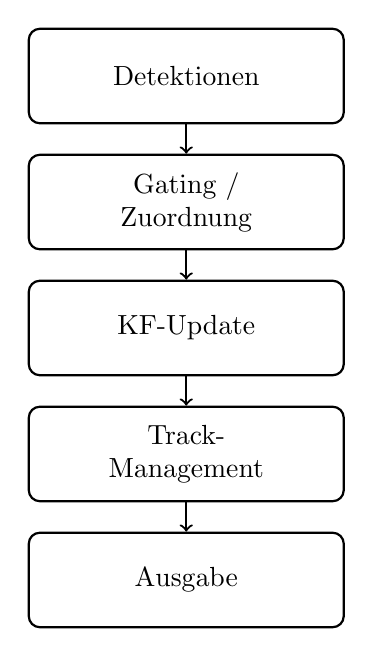
\begin{tikzpicture}[
      box/.style={
        rectangle,
        rounded corners,
        draw=black,
        thick,
        minimum width=4.0cm,
        minimum height=1.2cm,
        align=center
      },
      node distance=1.6cm
    ]

    % Nodes (vertical chain)
    \node[box] (det) {Detektionen};
    \node[box, below of=det] (gate) {Gating /\\ Zuordnung};
    \node[box, below of=gate] (kf) {\ac{KF}-Update};
    \node[box, below of=kf] (manage) {Track-\\Management};
    \node[box, below of=manage] (out) {Ausgabe};

    % Arrows
    \draw[->, thick] (det) -- (gate);
    \draw[->, thick] (gate) -- (kf);
    \draw[->, thick] (kf) -- (manage);
    \draw[->, thick] (manage) -- (out);

  \end{tikzpicture}
  \caption{Ablauf der Objektverfolgung.}
  \label{fig:tracking_flow}
\end{figure}

\section{Test und Ergebnis}
\label{sec:ergebnis_tracking}

\texttt{ids\_probe.py} beobachtet das Marker-Topic \texttt{tracks\_markers} und führt ein Lebensdauerkonto pro Track-ID. Für jede Spur werden Geburt und Abschluss (bei Leerlauf länger als \texttt{idle\_timeout}) gezählt, aktive sowie abgeschlossene mittlere Lebensdauern berechnet und die Geburts- bzw. Abschlussrate pro Minute ausgegeben. Der Skript läuft als eigener \ac{ROS}~2-Node, greift auf die bestehenden Topics zu und liefert so eine objektive Einschätzung der ID-Stabilität. Alle zugehörigen Auswerteskripte befinden sich zentral im digitalen Anhang (Abschnitt~\ref{anhang:skripte}).

Die Messergebnisse der Verifikation sind in Abschnitt~\ref{gerade_strecke} zusammengestellt.

\section{Zusammenfassung}
Der implementierte Tracker auf Basis eines 2D-Kalman-Filters und des Ungarischen Algorithmus gewährleistet eine konsistente Verfolgung der detektierten Objekte. Durch geeignetes Gating und Track-Management werden Fehlassoziationen minimiert und kurzzeitige Verdeckungen überbrückt. Damit ist die algorithmische Verarbeitungskette vollständig beschrieben.

Das folgende Kapitel widmet sich der Integration dieser Komponenten in die bestehende Softwareumgebung und Benutzeroberfläche des Versuchsträgers.